\documentclass{article}
\usepackage[margin=1in, a4paper]{geometry}
\usepackage[utf8]{inputenc}
\usepackage{mathtools}
%\usepackage{amsmath}
\usepackage{enumitem}
\usepackage{fancyhdr}
% labeled arrays
\usepackage{blkarray}
% diagrams
\usepackage{tikz}
% quotes
\usepackage{csquotes}
% graphics
\usepackage{graphicx}
% fix figure positions
\usepackage{float}
% add margins to captions
\usepackage[margin=1in]{caption}
% turn off hyphens
\usepackage[none]{hyphenat}
% links
\usepackage[hidelinks]{hyperref}
% edit verbatim
\usepackage{fancyvrb}
% mutliple columns
\usepackage{multicol}

\lhead{Evan Kohilas}
\rhead{COMP4121 - Project}
\pagestyle{fancy}
\title{COMP4121}
% sub counting
%\numberwithin{equation}{section}
% automatic newlines
\usepackage{parskip}

\begin{document}

\title{
    {\textbf{Contextual Text Prediction\\using Hidden Markov Models}}\\
    {University of New South Wales}\\
    {COMP4121 -- Project}
}
\author{Evan Kohilas -- 20th November 2017}
\date{}
\maketitle

\begin{abstract}
    General text prediction is often done through analysis of paired words,
    where suggested words are those which are most commonly used or followed.
    While these models can be useful in predicting a sender's text, they often
    lack understanding in the context of the receiver in a conversation. In this
    paper, we explore the different usages of Hidden Markov Models where we
    attempt to predict a sender's next word from the predicted states given the
    sender's current input as the observed states.
\end{abstract}

\section{Introduction}
Most modern text prediction attempts to predict words by searching models of
ranked words for the most probable following word. Often these models are
combined with other algorithms to better model the sender. However because these
models do well in automatically completing words or predicting common words,
they can lack meaning that is relevant to the current conversation, or the
receiver.

\begin{figure}[H]
    \centering
    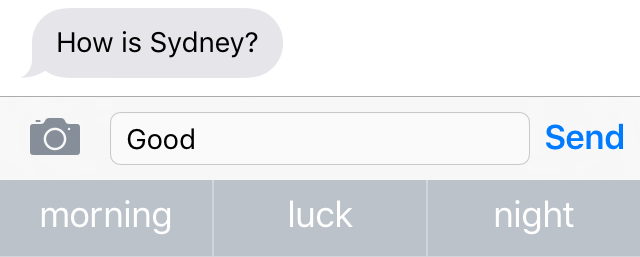
\includegraphics[width=0.5\textwidth]{sydney.png}
    \caption{Example of iOS predictive text lacking context.}
\end{figure}

Using Hidden Markov Models and algorithms such as the Viterbi Algorithm,
we will attempt to predict a sender's next word weighted using a corpus.
First we will describe HMMs and Viterbi and then further on we will describe our
process of exploring the different methods of weighing such a model.

\subsection{Markov Models}
Markov models are used to model systems on random factors. Such model's future
states are predicted using previous states.

One example of a Markov model is to parse a corpus of data, keeping track of
the probabilities of words that follow each other. Given such a model, we can
then follow the probabilities in a chain like manner to obtain the most likely
sentence, or factor in different probabilities to generate random likely
sentences.

The module \href{https://github.com/jsvine/markovify}{``\underline{markovify}''} has implemented this model using a corpus of Sherlock
Holmes books, and can generate sentences such as:
\begin{displayquote}
    ``It cost me something in foolscap, and I had no idea that
    he was a man of evil reputation among women.''
\end{displayquote}

\subsection{Hidden Markov Models}
Unlike normal Markov models where there is only one state that is visible to
the user, a Hidden Markov Model exhibits an additional state that is
unobserved, and is thus hidden.

To put it more simply, a HMM describes situations where the events that occur
cannot be accurately observed, but the probabilities of the actual events
occurring, and the probabilities of the inaccuracies are known.

The hidden events can thus be deduced using these probabilities, and thus the
hidden states can be estimated, or used to predict future hidden states.

One example is trying to predict the state that a person might currently be
exhibiting, given the person's previous medical observations.

\tikzstyle{state}=[circle, draw, align=center, minimum size = 1.3cm]%, font=\footnotesize]
\tikzstyle{prob}=[circle, draw, minimum size = 1.3cm, font=\footnotesize]
\tikzstyle{start}=[state, double]
\tikzstyle{probstart}=[start, double]
\tikzstyle{edge}=[<-, very thin]
\tikzstyle{lightedge}=[<-, dotted]
\tikzstyle{mainstate}=[state,thick]
\tikzstyle{mainedge}=[<-, very thick]

\begin{figure}[H]
    \centering
    % probabilities
    \begin{tikzpicture}[]
        % start
        \node[probstart] (start) at (0,1) {start};
        % 1st column
        \node[prob] (h) at (3,2) {Healthy}
            edge [edge] node [yshift=10pt] {0.6} (start)
            edge [<-, loop above, looseness=5] node {0.7} (h)
        ;
        \node[prob] (f) at (3,0) {Fever}
            edge [edge] node [yshift=-10pt] {0.4} (start)
            edge [<-, loop below, looseness=5] node {0.6} (f)
            edge [->, bend left=30] node [xshift=-10pt] {0.3} (h)
            edge [<-, bend right=30] node [xshift=-10pt] {0.4} (h)
        ;
        % 2nd column
        \node[prob] (n) at (6, 2.5) {Normal}
            edge [lightedge] node [yshift=5pt, xshift=-8pt] {0.5} (h)
            edge [lightedge] node [yshift=-17pt, xshift=-8pt] {0.1} (f)
        ;
        \node[prob] (c) at (6, 1) {Cold}
            edge [lightedge] node [yshift=9pt, xshift=-8pt] {0.4} (h)
            edge [lightedge] node [yshift=-9pt, xshift=-8pt] {0.3} (f)
        ;
        \node[prob] (d) at (6, -0.5) {Dizzy}
            edge [lightedge] node [yshift=17pt, xshift=-8pt] {0.1} (h)
            edge [lightedge] node [yshift=-5pt, xshift=-8pt] {0.6} (f)
        ;
    \end{tikzpicture}
    \caption{
        A HMM probability diagram denoting the states and
        observations of a person.
    }
\end{figure}

Using a HMM, we can attempt to predict a person's current health using only the
observations that can be seen from the outside. We do this by finding the most
likely state given each current observation. This can be done using the Viterbi
Algorithm.

\subsection{The Viterbi Algorithm}
The Viterbi Algorithm is a dynamic programming algorithm for finding the most
likely sequence of hidden states (called the Viterbi Path).

The algorithm is given a set of observed states $O$,
a set of initial probabilities, a set of transitional probabilities
where $P(x \rightarrow y)$ denotes the chance of going from $x$ to $y$, and a
set of observational probabilities $P(x\ |\ y)$ which denote the chance that
$x$ happens given $y$.

The algorithm works by finding:
\begin{align*}
    \max \{ (P(S_{t-1})P(S_{t-1} \rightarrow S_{t})P(O_{t}\ |\ S_{t}))
        : \forall \ S\}\ \forall \ t
\end{align*}
and upon conclusion, returns which hidden states were the most likely occur.

\begin{figure}[H]
    \centering
    \begin{tikzpicture}[]
        % start
        \node[start] (start) at (0,2) {start};
        % 1st column
        \node               at (2,4) {Normal};
        \node[mainstate] (sp1) at (2,3) {H\\\tiny0.3}
            edge[mainedge] (start);
        \node[state] (sr1) at (2,1) {F\\\tiny0.04}
            edge[edge] (start);
        \node at (2,0) {$t_1$};
        % 2nd column
        \node               at (4,4) {Cold};
        \node[mainstate] (sp2) at (4, 3) {H\\\tiny0.084}
            edge[mainedge] (sp1)
            edge[edge] (sr1)
        ;
        \node[state] (sr2) at (4, 1) {F\\\tiny0.027}
            edge[edge] (sp1)
            edge[edge] (sr1)
        ;
        \node at (4, 0) {$t_2$};
        % 3nd column
        \node               at (6,4) {Dizzy};
        \node[state] (sp3) at (6, 3) {H\\\tiny0.00588}
            edge[edge] (sp2)
            edge[edge] (sr2)
        ;
        \node[mainstate] (sr3) at (6, 1) {F\\\tiny0.00972}
            edge[mainedge] (sp2)
            edge[edge] (sr2)
        ;
        \node at (6, 0) {$t_3$};
    \end{tikzpicture}
    \caption{
        This trellis diagram of the HMM in Figure 2 shows the sequence of
        states with the maximum probabilities, giving a hidden state for each
        observed state. Thus, we can conclude that the person was Healthy on
        day 1 and 2, but had a Fever on day 3.
    }
\end{figure}

\section{Methods and Results}
We first explore generating Markov chains from our given data. This consisted
of breaking up sentences into words which were then parsed into a 2D dictionary
which stored the number of times word $w_1$ was followed by word $w_2$.

From this, for any given $w_1$, we can then find what the next most likely
following word would be. In our data, we found that a sentence has a \sim9\%
chance to start with `I', and a \sim2\% chance to start with `oh', `and',
`yeah', or `its'. We also found that the most likely sentence from beginning to
end is ``I have a good''.

\subsection{Data}
All the data used in this report was collected from a single facebook chatroom
consisting of over 100 users and over 100,000 messages over a period of almost
1 year.

The data was then extracted and processed in a simple manner where
(\textsc{\char13}) and (\textsc{'}) were removed, with all data converted to
lower case. Finally, every sequence of one of more Unicode letters are then
treated as words. This simple method is used to deal with words such as
``it's'' and ``I'm'', which help greatly in this simple method.

We then convert these words into bigrams, where a ``BEGIN'' token is treated as
the first word. Thus, the sentence ``Who's a good boy?'' becomes:
(BEGIN, `whos'), (`whos', `a'), (`a', `good'), (`good', `boy').

Afterwards, we generate the 2D dictionary (or identically, a matrix)
using these bi-grams, incrementing for each time one is seen, but only doing so
when both words exist in our set of words. We do this so that we can unify our
data when it comes to using different corpuses.

In our implementation, we chose to ignore (`boy', END) as we would not like to
generate predictions with endings. We also chose to ignore any bi-grams which
contained words that only appeared once. This was done to remove any rare words
that would not have a large effect. More importantly, this step reduces our
total different word count from \sim28,000 words to \sim 14,000 words, which
greatly helps with the processing of the Viterbi algorithm.

Finally, we normalise our matrix by dividing each row $w_1$ by the total number
of words that follow $w_1$, thus giving us the chance that $w_1$ follows $w_2$.
Further, to ensure we don't ignore words that are never followed, we add
$\frac{1}{S}$ to each element in the matrix (where $S$ is the total number of
different words).

Additionally, we can also generate multiple matrices consisting of only the
sender's messages, or all but the sender's.

\subsubsection{Test Data}
To test our models, we use a sample of 35 various sentences:
\begin{itemize}
    \setlength\itemsep{-0.5ex}
    \item ``Are you''
    \item ``Because''
    \item ``Do you''
    \item ``Do you wanna''
    \item ``Do you want to''
    \item ``Evan''
    \item ``How about''
    \item ``How often''
    \item ``I''
    \item ``I am''
    \item ``I am so excited for''
    \item ``I don't''
    \item ``I feel like''
    \item ``I forgot''
    \item ``I'll be''
    \item ``I love''
    \item ``I'm''
    \item ``I'm not''
    \item ``I'm so''
    \item ``Is there''
    \item ``Is this a possible''
    \item ``I think I have''
    \item ``I think I've''
    \item ``It is up to''
    \item ``It's up to''
    \item ``I want''
    \item ``I want to eat''
    \item ``I want you to''
    \item ``I will be''
    \item ``The''
    \item ``The best''
    \item ``The only''
    \item ``What are you''
    \item ``What is''
    \item ``What's''
\end{itemize}
These sentences were picked to give the models a variety of possible states
to consider and test. Some were picked as a comparison to the iOS text
prediction while others were picked specifically for testing the model.
We will analyse the performance of each model on how well each predicted word
fits in the sentence.

\subsection{Prediction using HMM}
Next, we explored the use of HMM's on our matrices, by feeding in the above
matrix into the Viterbi algorithm.
The idea behind text prediction using a HMM is to use the sender's current
sentence as the observed state, letting the HMM generate a hidden sentence
which it thinks is what the sender could actually be saying.

We do this through giving the model a probability matrix like the one above,
which it then uses to find the most likely word that follows the previous word,
and is related to the given observed state.

In effect, the transitional probability matrix generates what the sender is
likely to say, while the observation probabilities matrix weighs the hidden
state in accordance to the observed state, which could act as what the sender
should say. Another way of looking at this would be, given what the sender has
typed, what's the most likely thing that the receiver would say next?

Different given matrices would thus produce different hidden states. Finally, a
variety of methods can be used for prediction of the next word given the last
word of the hidden state.

\subsubsection{Standard HMM}
In this configuration of the HMM, we fed the standard Viterbi algorithm a
probability matrix consisting of all the messages as the observational and
transitional probabilities. The sender's predicted word was then found by
taking the final word from the hidden state and finding it's most likely
following word.

In effect, the model's hidden states are generated using the most likely words,
weighted by the chance that the current word is followed by the observed word.

\textbf{Results}\\
Below are the results using the Standard HMM. The words in round brackets are
the final hidden states, while the word in square brackets is the prediction
for that current line.

Only 6 from the 35 results were found to be reasonable predictions.
\begin{multicols}{3}
\begin{Verbatim}[fontsize=\footnotesize]
(roses, are)
are you [you]

(its)
because [a]

(how, do)
do you [you]

(how, do, u)
do you wanna [have]

(how, do, you, want)
do you want to [to]

(thx)
evan [evan]

(idk, what)
how about [is]

(idk, how)
how often [to]

(yeah)
i [i]

(yeah, i)
i am [have]

(yeah, i, think, reliably, excited)
i am so excited for [for]

(yeah, i)
i dont [have]

(yeah, i, feel)
i feel like [like]

(yeah, i)
i forgot [have]

(okok, ill)
ill be [be]

(yeah, i)
i love [have]

(yeah)
im [i]

(bahaha, im)
im not [not]

(bahaha, im)
im so [not]

(this, is)
is there [a]

(this, is, such, as)
is this a possible [a]

(yeah, i, wish, i)
i think i have [have]

(yeah, i, think)
i think ive [i]


(intended, audience, spinning, up)
it is up to [to]

(nah, ended, up)
its up to [to]

(yeah, i)
i want [have]

(if, you, want, to)
i want to eat [be]

(yeah, i, dont, want)
i want you to [to]

(omfg, dj, will)
i will be [be]

(and)
the [i]

(whats, the)
the best [same]

(whats, the)
the only [same]

(idk, why, are)
what are you [you]

(wait, what)
what is [is]

(wait)
whats [what]
\end{Verbatim}
\end{multicols}


While this model has this resulted in somewhat reasonable results, the model
was ``lagging'' as the hidden states were weighed on not what should be
next word, but what was the current observed word, and thus when the model was
predicting sentences well, it would predict the same word as the last observed
word.

\subsubsection{Shifted HMM}
Our next attempt consists of altering the Viterbi algorithm to be
shifted along by one word, such that current hidden state is weighed on the
next state of the observed states. The final state is then generated by
finding the most likely word to follow the previous state, given the last
observation.

This method produced varying results, but it could be said that it was better than the standard HMM as the ``lagging'' had disappeared. However, it was still lacking as the final state was not entirely a word that was to follow given that it was generated using the previous state, and the final observed word, when instead we would rather generate a word that is to follow
our last.

\textbf{Results}\\
Below are the results using a Shifted HMM. Taking the words from the final
state or taking the final state's most likely following word (in square brackets)
only results in about 7 reasonable results.
\begin{multicols}{3}
\begin{Verbatim}[fontsize=\footnotesize]
(what, are)
are you [you]

(a)
because [good]

(what, are)
do you [you]

(thank, u, dont)
do you wanna [have]

(thank, u, go, back)
do you want to [to]

(a)
evan [good]

(idk, what)
how about [is]

(becuase, you)
how often [can]

(a)
i [good]

(why, i)
i am [have]

(i, am, currently, stands, up)
i am so excited for [to]

(i, just)
i dont [a]

(blobs, feel, looks)
i feel like [like]

(i, totally)
i forgot [not]

(ill, probably)
ill be [not]

(i, would)
i love [be]

(a)
im [good]

(but, its)
im not [a]

(ohhhhh, ok)
im so [i]

(rite, rite)
is there [in]

(deserve, such, as, a)
is this a possible [good]

(i, wish, i, dont)
i think i have [have]

(i, think, so)
i think ive [i]


(audience, spinning, up, going)
it is up to [to]

(ended, up, going)
its up to [to]

(i, dont)
i want [have]

(i, want, to, go)
i want to eat [to]

(i, did, you, want)
i want you to [to]

(radio, will, probably)
i will be [not]

(a)
the [good]

(loot, loot)
the best [could]

(octopus, merge)
the only [afterwards]

(you, can, do)
what are you [you]

(wait, what)
what is [is]

(a)
whats [good]
\end{Verbatim}
\end{multicols}

\pagebreak
\subsubsection{Similarity HMM}
In the ``Similarity'' HMM, we alter the HMM so that instead of weighting a word
in each hidden state based on how well it is followed the observed word, we
would like to instead generate words that follow the last hidden state, but are
also the most similar to the observed states.

Instead of letting our observational matrix be a mapping of how strongly word
$w_1$ is followed by $w_2$ we instead let our matrix map the similarity between
words $w_1$ and $w_2$.

Two words are said to be similar if the percentage of words that are followed
by $w_1$ is similar to the percentage of those words that also follow $w_2$. To
do this, we can use the cosine similarity between each column vector of the
matrix where where each entry is the number of times $w_1$ is followed
by $w_2$.

By using this method with each given hidden state, a word is generated using
the previous word and the words similarity to the given observed word.
Finally, we can then take the final word from the hidden states and find it's
next most likely following word.

\textbf{Results}\\
Below are the results using the first the HMM. 14 from the 35 results were found
to be reasonable predictions.
\begin{multicols}{3}
\begin{Verbatim}[fontsize=\footnotesize]
(are, you)
are you [can]

(i)
because [have]

(do, you)
do you [can]

(do, you, can)
do you wanna [i]

(do, you, want, to)
do you want to [be]

(i)
evan [have]

(what, about)
how about [it]

(i, have)
how often [a]

(i)
i [have]

(i, think)
i am [i]

(i, think, so, excited, for)
i am so excited for [the]

(i, have)
i dont [a]

(i, have, a)
i feel like [good]

(i, think)
i forgot [i]

(i, do)
ill be [you]

(i, think)
i love [i]

(i)
im [have]

(im, not)
im not [a]

(im, not)
im so [a]

(is, a)
is there [good]

(is, this, is, a)
is this a possible [good]

(i, think, i, have)
i think i have [a]

(i, think, i)
i think ive [have]


(i, was, going, to)
it is up to [be]

(im, going, to)
its up to [be]

(i, have)
i want [a]

(i, want, to, be)
i want to eat [a]

(i, think, its, a)
i want you to [good]

(i, would, be)
i will be [a]

(i)
the [have]

(the, same)
the best [time]

(i, have)
the only [a]

(what, are, you)
what are you [can]

(what, is)
what is [a]

(i)
whats [have]
\end{Verbatim}
\end{multicols}

While these results are reasonable, they lack depth due to the fact that the
most likely following word in most cases are common words such as ``good'',
``a'', and ``i''.

We give a second alteration of this model similar to the shifted HMM where
after the final iteration, another word is generated using the current final
hidden word, given words that could follow the final observed word.

\pagebreak
\textbf{Results}\\
Below are the results using the second version of the Similarity HMM. 6 from
the 35 results were found to be reasonable predictions.
\begin{multicols}{3}
\begin{Verbatim}[fontsize=\footnotesize]

(are, you, are)
are you [are]

(i, just)
because [just]

(do, you, are)
do you [are]

(do, you, can, u)
do you wanna [u]

(do, you, want, to, go)
do you want to [go]

(alex, <redacted last name>)
evan [<redacted last name>]

(i, dont, worry)
how about [worry]

(how, much, more)
how often [more]

(i, think)
i [think]

(i, think, i)
i am [i]

(i, think, so, excited, for, me)
i am so excited for [me]

(i, think, i)
i dont [i]

(i, think, i, feel)
i feel like [feel]

(i, think, i)
i forgot [i]

(i, have, to)
ill be [to]

(i, think, i)
i love [i]

(i, think)
im [think]

(im, going, to)
im not [to]

(im, so, im)
im so [im]

(is, this, is)
is there [is]

(is, that, too, long, as)
is this a possible [as]

(i, think, i, think, i)
i think i have [i]

(i, think, i, think)
i think ive [think]

(i, was, going, to, go)
it is up to [go]

(im, going, to, go)
its up to [go]

(i, think, i)
i want [i]

(i, want, to, go, to)
i want to eat [to]

(i, dont, want, to, go)
i want you to [go]

(i, dont, go, to)
i will be [to]

(this, is)
the [is]

(the, best, keanu)
the best [keanu]

(i, think, i)
the only [i]

(what, are, you, are)
what are you [are]

(what, is, this)
what is [this]

(i, know)
whats [know]

\end{Verbatim}
\end{multicols}

While the results of this method lacked, the algorithm behind it was useful in
generating predictions upon being given different datasets, such that different
predictions that would be weighted on different factors.

\pagebreak
\textbf{Results}\\
Below are the results of using the Similarity HMM where only a set of the
sender's messages were passed as the transitional matrix. 14 from the 35 results
were found to be reasonable predictions. More importantly, these predictions
were found useful as they had more depth (possibly due to the reduced dataset).
% i yeah nice lol again works python obj obj equals
\begin{multicols}{3}
\begin{Verbatim}[fontsize=\footnotesize]
(are, you, can)
are you [can]

(im, homesick)
because [homesick]

(do, you, can)
do you [can]

(do, you, can, i)
do you wanna [i]

(do, you, want, to, get)
do you want to [get]

(its, name)
evan [name]

(what, im, talking)
how about [talking]

(i, need, to)
how often [to]

(i, think)
i [think]

(i, think, i)
i am [i]

(i, think, so, much, more, syntax)
i am so excited for [syntax]

(i, think, i)
i dont [i]

(i, think, i, feel)
i feel like [feel]

(i, think, i)
i forgot [i]

(i, have, to)
ill be [to]

(i, think, alex)
i love [alex]

(i, think)
im [think]

(im, glad, youre)
im not [youre]

(its, not, hungry)
im so [hungry]

(is, there, right)
is there [right]

(is, such, a, crime, as)
is this a possible [as]

(i, think, i, think, you)
i think i have [you]

(i, think, thats, what)
i think ive [what]

(i, was, going, to, get)
it is up to [get]

(im, trying, to, get)
its up to [get]

(i, think, you)
i want [you]

(i, need, to, do, you)
i want to eat [you]

(i, wonder, if, you, want)
i want you to [want]

(i, dont, get, to)
i will be [to]

(i, think)
the [think]

(the, same, the)
the best [the]

(the, rarest, items)
the only [items]

(what, are, you, can)
what are you [can]

(what, is, this)
what is [this]

(i, know)
whats [know]
\end{Verbatim}
\end{multicols}

\subsubsection{Reverse HMM}
In this configuration of the HMM, we fix the issue of our previous HMM which
was generating words that would would be followed by those in our observed
states by passing in a transposed observation matrix into the Viterbi
algorithm.

This would instead mean that our HMM would look for the most likely following
the previous, given by the most common word that would follow the one in the
observed state. We then take the last word in the hidden state as our predicted
word.

\pagebreak
\textbf{Results}\\
Below are the results using the Reverse HMM. 26 from the 35 results were found
to be reasonable predictions.
%``I just a good luck with the same time'' was returned upon recursive feeding.
\begin{multicols}{3}
\begin{Verbatim}[fontsize=\footnotesize]

(you, can)
are you [can]

(i)
because [i]

(i, have)
do you [have]

(i, can, do)
do you wanna [do]

(i, have, to, be)
do you want to [be]

(i)
evan [i]

(do, it)
how about [it]

(i, have)
how often [have]

(just)
i [just]

(can, i)
i am [i]

(have, a, good, for, the)
i am so excited for [the]

(dont, have)
i dont [have]

(was, like, a)
i feel like [a]

(have, to)
i forgot [to]

(have, a)
ill be [a]

(do, it)
i love [it]

(not)
im [not]

(not, a)
im not [a]

(so, i)
im so [i]

(it, was)
is there [was]

(it, is, good, to)
is this a possible [to]

(can, i, have, a)
i think i have [a]

(can, i, got)
i think ive [got]

(is, it, to, be)
it is up to [be]

(not, to, be)
its up to [be]

(have, to)
i want [to]

(have, to, do, it)
i want to eat [it]

(have, to, get, the)
i want you to [the]

(can, be, a)
i will be [a]

(same)
the [same]

(same, thing)
the best [thing]

(same, thing)
the only [thing]

(do, you, can)
what are you [can]

(is, a)
what is [a]

(the)
whats [the]

\end{Verbatim}
\end{multicols}

This model found to give the best results, however unlike the similarity model,
it did not produce variably different results on using different datasets.

\section{Discussion and Conclusion}
In conclusion, we found that the ``Reverse'' Hidden Markov Model proved to be
useful in generating useful predictive text, however the ``Similarity'' Hidden
Markov Model can also prove to be useful when in use with multiple datasets,
which could further be curated.

It may have been possible that better results could have risen if better post
processing to the data was applied. Additionally, more tests could have been
performed for each type of model, especially where different types of datasets
were given, such as limiting a dataset to a certain time frame to provide time
contextual predictions.

In summary, exploring Hidden Markov Models for the use of Text Prediction proved to be useful and worth investigating in a greater depth and with more time.
\end{document}
